\documentclass[]{article}
\usepackage{lmodern}
\usepackage{amssymb,amsmath}
\usepackage{ifxetex,ifluatex}
\usepackage{fixltx2e} % provides \textsubscript
\ifnum 0\ifxetex 1\fi\ifluatex 1\fi=0 % if pdftex
  \usepackage[T1]{fontenc}
  \usepackage[utf8]{inputenc}
\else % if luatex or xelatex
  \ifxetex
    \usepackage{mathspec}
  \else
    \usepackage{fontspec}
  \fi
  \defaultfontfeatures{Ligatures=TeX,Scale=MatchLowercase}
\fi
% use upquote if available, for straight quotes in verbatim environments
\IfFileExists{upquote.sty}{\usepackage{upquote}}{}
% use microtype if available
\IfFileExists{microtype.sty}{%
\usepackage[]{microtype}
\UseMicrotypeSet[protrusion]{basicmath} % disable protrusion for tt fonts
}{}
\PassOptionsToPackage{hyphens}{url} % url is loaded by hyperref
\usepackage[unicode=true]{hyperref}
\hypersetup{
            pdftitle={Cost-Effectiveness and Decision Modeling in R},
            pdfauthor={The DARTH workgroup},
            pdfborder={0 0 0},
            breaklinks=true}
\urlstyle{same}  % don't use monospace font for urls
\usepackage[margin=1in]{geometry}
\usepackage{longtable,booktabs}
% Fix footnotes in tables (requires footnote package)
\IfFileExists{footnote.sty}{\usepackage{footnote}\makesavenoteenv{long table}}{}
\usepackage{graphicx,grffile}
\makeatletter
\def\maxwidth{\ifdim\Gin@nat@width>\linewidth\linewidth\else\Gin@nat@width\fi}
\def\maxheight{\ifdim\Gin@nat@height>\textheight\textheight\else\Gin@nat@height\fi}
\makeatother
% Scale images if necessary, so that they will not overflow the page
% margins by default, and it is still possible to overwrite the defaults
% using explicit options in \includegraphics[width, height, ...]{}
\setkeys{Gin}{width=\maxwidth,height=\maxheight,keepaspectratio}
\IfFileExists{parskip.sty}{%
\usepackage{parskip}
}{% else
\setlength{\parindent}{0pt}
\setlength{\parskip}{6pt plus 2pt minus 1pt}
}
\setlength{\emergencystretch}{3em}  % prevent overfull lines
\providecommand{\tightlist}{%
  \setlength{\itemsep}{0pt}\setlength{\parskip}{0pt}}
\setcounter{secnumdepth}{0}
% Redefines (sub)paragraphs to behave more like sections
\ifx\paragraph\undefined\else
\let\oldparagraph\paragraph
\renewcommand{\paragraph}[1]{\oldparagraph{#1}\mbox{}}
\fi
\ifx\subparagraph\undefined\else
\let\oldsubparagraph\subparagraph
\renewcommand{\subparagraph}[1]{\oldsubparagraph{#1}\mbox{}}
\fi

% set default figure placement to htbp
\makeatletter
\def\fps@figure{htbp}
\makeatother

\usepackage{etoolbox}
\makeatletter
\providecommand{\subtitle}[1]{% add subtitle to \maketitle
  \apptocmd{\@title}{\par {\large #1 \par}}{}{}
}
\makeatother

\title{Cost-Effectiveness and Decision Modeling in R}
\providecommand{\subtitle}[1]{}
\subtitle{SA Markov Model Exercise}
\author{The DARTH workgroup}
\date{}

\begin{document}
\maketitle

Developed by the Decision Analysis in R for Technologies in Health
(DARTH) workgroup:

Fernando Alarid-Escudero, PhD (1)

Eva A. Enns, MS, PhD (2)

M.G. Myriam Hunink, MD, PhD (3,4)

Hawre J. Jalal, MD, PhD (5)

Eline M. Krijkamp, MSc (3)

Petros Pechlivanoglou, PhD (6,7)

Alan Yang, MSc (7)

In collaboration of:

\begin{enumerate}
\def\labelenumi{\arabic{enumi}.}
\tightlist
\item
  Division of Public Administration, Center for Research and Teaching in
  Economics (CIDE), Aguascalientes, Mexico
\item
  University of Minnesota School of Public Health, Minneapolis, MN, USA
\item
  Erasmus MC, Rotterdam, The Netherlands
\item
  Harvard T.H. Chan School of Public Health, Boston, USA
\item
  University of Pittsburgh Graduate School of Public Health, Pittsburgh,
  PA, USA
\item
  University of Toronto, Toronto ON, Canada
\item
  The Hospital for Sick Children, Toronto ON, Canada
\end{enumerate}

Please cite our publications when using this code:

\begin{itemize}
\item
  Jalal H, Pechlivanoglou P, Krijkamp E, Alarid-Escudero F, Enns E,
  Hunink MG. An Overview of R in Health Decision Sciences. Med Decis
  Making. 2017; 37(3): 735-746.
  \url{https://journals.sagepub.com/doi/abs/10.1177/0272989X16686559}
\item
  Alarid-Escudero F, Krijkamp EM, Enns EA, Yang A, Hunink MGM
  Pechlivanoglou P, Jalal H. Cohort State-Transition Models in R: A
  Tutorial. arXiv:200107824v2. 2020:1-48.
  \url{http://arxiv.org/abs/2001.07824}
\item
  Krijkamp EM, Alarid-Escudero F, Enns EA, Jalal HJ, Hunink MGM,
  Pechlivanoglou P. Microsimulation modeling for health decision
  sciences using R: A tutorial. Med Decis Making. 2018;38(3):400--22.
  \url{https://journals.sagepub.com/doi/abs/10.1177/0272989X18754513}
\item
  Krijkamp EM, Alarid-Escudero F, Enns E, Pechlivanoglou P, Hunink MM,
  Jalal H. A Multidimensional Array Representation of State-Transition
  Model Dynamics. Med Decis Making. 2020 Online first.
  \url{https://doi.org/10.1177/0272989X19893973}
\end{itemize}

Copyright 2017, THE HOSPITAL FOR SICK CHILDREN AND THE COLLABORATING
INSTITUTIONS. All rights reserved in Canada, the United States and
worldwide. Copyright, trademarks, trade names and any and all associated
intellectual property are exclusively owned by THE HOSPITAL FOR Sick
CHILDREN and the collaborating institutions. These materials may be
used, reproduced, modified, distributed and adapted with proper
attribution.

\section{Exercise I: Construct a Markov Model of the Sick-Sicker Disease
(COMPLETED)}\label{exercise-i-construct-a-markov-model-of-the-sick-sicker-disease-completed}

In this exercise, we will model a hypothetical disease that affects
individuals with an average age of 25 years and results in increased
mortality, increased healthcare costs, and reduced quality of life. The
disease has two levels; affected individuals initially become sick but
can subsequently progress and become sicker. Two alternative strategies
exist for this hypothetical disease: a no-treatment and a treatment
strategy. Under the treatment strategy, individuals in the sick and
sicker states are treated until they recover (only if sick; individuals
in the sicker state cannot recover) or die. The cost of the treatment is
additive to the baseline healthcare costs of being sick or sicker. The
treatment improves quality of life for those individuals who are sick
but has no impact on the quality of life of those who are sicker.
Unfortunately, it is not possible to reliably differentiate between
people in the sick and sicker states, so treatment cannot be targeted to
only those in the sick state. You are asked to evaluate the
cost-effectiveness of the treatment.

To model this disease, we will rely on a state-transition cohort model,
called the Sick-Sicker model, first described by Enns et al. The
Sick-Sicker model consists of four health states: Healthy (H), two
disease states, Sick (S1) and Sicker (S2), and Dead (D) (Figure 1). All
individuals start in the Healthy state. Over time, healthy individuals
may develop the disease and can progress to S1. Individuals in S1 can
recover (return to state H), progress further to S2 or die. Individuals
in S2 cannot recover (i.e.~cannot transition to either S1 or H).
Individuals in H have a baseline probability of death; individuals in S1
and S2 experience increased mortality compared to those in the H state,
given in terms of hazard ratios. These ratios are used to calculate the
probabilities of dying when in S1 and S2.

\begin{figure}

{\centering 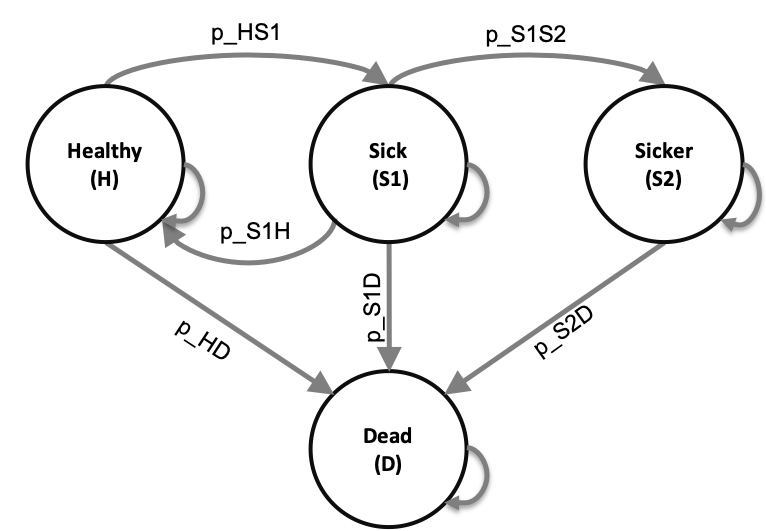
\includegraphics[width=1\linewidth]{sick_sicker_diagram} 

}

\caption{Schematic representation of the Sick-Sicker model}\label{fig:unnamed-chunk-1}
\end{figure}

\subsection{Tasks (COMPLETED)}\label{tasks-completed}

\begin{enumerate}
\def\labelenumi{\arabic{enumi}.}
\item
  Build the cohort state transition model in \texttt{R} for no treatment
  and treatment strategies.
\item
  Plot the survival curve for the cohort under no treatment.
\item
  Estimate the cost-effectiveness of treatment vs no-treatment.
\item
  Create a cost-effectiveness table with all results of interest.
\end{enumerate}

\textbf{Table I: Input parameters}

\begin{longtable}[]{@{}llc@{}}
\toprule
\begin{minipage}[b]{0.47\columnwidth}\raggedright\strut
\textbf{Parameter}\strut
\end{minipage} & \begin{minipage}[b]{0.18\columnwidth}\raggedright\strut
\textbf{R name}\strut
\end{minipage} & \begin{minipage}[b]{0.20\columnwidth}\centering\strut
\textbf{Value}\strut
\end{minipage}\tabularnewline
\midrule
\endhead
\begin{minipage}[t]{0.47\columnwidth}\raggedright\strut
Time horizon\strut
\end{minipage} & \begin{minipage}[t]{0.18\columnwidth}\raggedright\strut
\texttt{n\_t}\strut
\end{minipage} & \begin{minipage}[t]{0.20\columnwidth}\centering\strut
30 years\strut
\end{minipage}\tabularnewline
\begin{minipage}[t]{0.47\columnwidth}\raggedright\strut
Cycle length\strut
\end{minipage} & \begin{minipage}[t]{0.18\columnwidth}\raggedright\strut
\strut
\end{minipage} & \begin{minipage}[t]{0.20\columnwidth}\centering\strut
1 year\strut
\end{minipage}\tabularnewline
\begin{minipage}[t]{0.47\columnwidth}\raggedright\strut
Names of health states\strut
\end{minipage} & \begin{minipage}[t]{0.18\columnwidth}\raggedright\strut
\texttt{v\_n}\strut
\end{minipage} & \begin{minipage}[t]{0.20\columnwidth}\centering\strut
H, S1, S2, D\strut
\end{minipage}\tabularnewline
\begin{minipage}[t]{0.47\columnwidth}\raggedright\strut
Annual discount rate (costs/QALYs)\strut
\end{minipage} & \begin{minipage}[t]{0.18\columnwidth}\raggedright\strut
\texttt{d\_r}\strut
\end{minipage} & \begin{minipage}[t]{0.20\columnwidth}\centering\strut
3\%\strut
\end{minipage}\tabularnewline
\begin{minipage}[t]{0.47\columnwidth}\raggedright\strut
Annual transition probabilities\strut
\end{minipage} & \begin{minipage}[t]{0.18\columnwidth}\raggedright\strut
\strut
\end{minipage} & \begin{minipage}[t]{0.20\columnwidth}\centering\strut
\strut
\end{minipage}\tabularnewline
\begin{minipage}[t]{0.47\columnwidth}\raggedright\strut
- Disease onset (H to S1), conditional on surviving\strut
\end{minipage} & \begin{minipage}[t]{0.18\columnwidth}\raggedright\strut
\texttt{p\_HS1}\strut
\end{minipage} & \begin{minipage}[t]{0.20\columnwidth}\centering\strut
0.15\strut
\end{minipage}\tabularnewline
\begin{minipage}[t]{0.47\columnwidth}\raggedright\strut
- Recovery (S1 to H), conditional on surviving\strut
\end{minipage} & \begin{minipage}[t]{0.18\columnwidth}\raggedright\strut
\texttt{p\_S1H}\strut
\end{minipage} & \begin{minipage}[t]{0.20\columnwidth}\centering\strut
0.5\strut
\end{minipage}\tabularnewline
\begin{minipage}[t]{0.47\columnwidth}\raggedright\strut
- Disease progression (S1 to S2) conditional on surviving, in the
time-homogeneous model\strut
\end{minipage} & \begin{minipage}[t]{0.18\columnwidth}\raggedright\strut
\texttt{p\_S1S2}\strut
\end{minipage} & \begin{minipage}[t]{0.20\columnwidth}\centering\strut
0.105\strut
\end{minipage}\tabularnewline
\begin{minipage}[t]{0.47\columnwidth}\raggedright\strut
Annual mortality\strut
\end{minipage} & \begin{minipage}[t]{0.18\columnwidth}\raggedright\strut
\strut
\end{minipage} & \begin{minipage}[t]{0.20\columnwidth}\centering\strut
\strut
\end{minipage}\tabularnewline
\begin{minipage}[t]{0.47\columnwidth}\raggedright\strut
- All-cause mortality (H to D)\strut
\end{minipage} & \begin{minipage}[t]{0.18\columnwidth}\raggedright\strut
\texttt{p\_HD}\strut
\end{minipage} & \begin{minipage}[t]{0.20\columnwidth}\centering\strut
0.005\strut
\end{minipage}\tabularnewline
\begin{minipage}[t]{0.47\columnwidth}\raggedright\strut
- Hazard ratio of death in S1 vs H\strut
\end{minipage} & \begin{minipage}[t]{0.18\columnwidth}\raggedright\strut
\texttt{hr\_S1}\strut
\end{minipage} & \begin{minipage}[t]{0.20\columnwidth}\centering\strut
3\strut
\end{minipage}\tabularnewline
\begin{minipage}[t]{0.47\columnwidth}\raggedright\strut
- Hazard ratio of death in S2 vs H\strut
\end{minipage} & \begin{minipage}[t]{0.18\columnwidth}\raggedright\strut
\texttt{hr\_S2}\strut
\end{minipage} & \begin{minipage}[t]{0.20\columnwidth}\centering\strut
10\strut
\end{minipage}\tabularnewline
\begin{minipage}[t]{0.47\columnwidth}\raggedright\strut
Annual costs\strut
\end{minipage} & \begin{minipage}[t]{0.18\columnwidth}\raggedright\strut
\strut
\end{minipage} & \begin{minipage}[t]{0.20\columnwidth}\centering\strut
\strut
\end{minipage}\tabularnewline
\begin{minipage}[t]{0.47\columnwidth}\raggedright\strut
- Healthy individuals\strut
\end{minipage} & \begin{minipage}[t]{0.18\columnwidth}\raggedright\strut
\texttt{c\_H}\strut
\end{minipage} & \begin{minipage}[t]{0.20\columnwidth}\centering\strut
\$2,000\strut
\end{minipage}\tabularnewline
\begin{minipage}[t]{0.47\columnwidth}\raggedright\strut
- Sick individuals in S1\strut
\end{minipage} & \begin{minipage}[t]{0.18\columnwidth}\raggedright\strut
\texttt{c\_S1}\strut
\end{minipage} & \begin{minipage}[t]{0.20\columnwidth}\centering\strut
\$4,000\strut
\end{minipage}\tabularnewline
\begin{minipage}[t]{0.47\columnwidth}\raggedright\strut
- Sick individuals in S2\strut
\end{minipage} & \begin{minipage}[t]{0.18\columnwidth}\raggedright\strut
\texttt{c\_S2}\strut
\end{minipage} & \begin{minipage}[t]{0.20\columnwidth}\centering\strut
\$15,000\strut
\end{minipage}\tabularnewline
\begin{minipage}[t]{0.47\columnwidth}\raggedright\strut
- Dead individuals\strut
\end{minipage} & \begin{minipage}[t]{0.18\columnwidth}\raggedright\strut
\texttt{c\_D}\strut
\end{minipage} & \begin{minipage}[t]{0.20\columnwidth}\centering\strut
\$0\strut
\end{minipage}\tabularnewline
\begin{minipage}[t]{0.47\columnwidth}\raggedright\strut
- Additional costs of sick individuals treated in S1 or S2\strut
\end{minipage} & \begin{minipage}[t]{0.18\columnwidth}\raggedright\strut
\texttt{c\_trt}\strut
\end{minipage} & \begin{minipage}[t]{0.20\columnwidth}\centering\strut
\$12,000\strut
\end{minipage}\tabularnewline
\begin{minipage}[t]{0.47\columnwidth}\raggedright\strut
Utility weights\strut
\end{minipage} & \begin{minipage}[t]{0.18\columnwidth}\raggedright\strut
\strut
\end{minipage} & \begin{minipage}[t]{0.20\columnwidth}\centering\strut
\strut
\end{minipage}\tabularnewline
\begin{minipage}[t]{0.47\columnwidth}\raggedright\strut
- Healthy individuals\strut
\end{minipage} & \begin{minipage}[t]{0.18\columnwidth}\raggedright\strut
\texttt{u\_H}\strut
\end{minipage} & \begin{minipage}[t]{0.20\columnwidth}\centering\strut
1.00\strut
\end{minipage}\tabularnewline
\begin{minipage}[t]{0.47\columnwidth}\raggedright\strut
- Sick individuals in S1\strut
\end{minipage} & \begin{minipage}[t]{0.18\columnwidth}\raggedright\strut
\texttt{u\_S1}\strut
\end{minipage} & \begin{minipage}[t]{0.20\columnwidth}\centering\strut
0.75\strut
\end{minipage}\tabularnewline
\begin{minipage}[t]{0.47\columnwidth}\raggedright\strut
- Sick individuals in S2\strut
\end{minipage} & \begin{minipage}[t]{0.18\columnwidth}\raggedright\strut
\texttt{u\_S2}\strut
\end{minipage} & \begin{minipage}[t]{0.20\columnwidth}\centering\strut
0.50\strut
\end{minipage}\tabularnewline
\begin{minipage}[t]{0.47\columnwidth}\raggedright\strut
- Dead individuals\strut
\end{minipage} & \begin{minipage}[t]{0.18\columnwidth}\raggedright\strut
\texttt{u\_D}\strut
\end{minipage} & \begin{minipage}[t]{0.20\columnwidth}\centering\strut
0.00\strut
\end{minipage}\tabularnewline
\begin{minipage}[t]{0.47\columnwidth}\raggedright\strut
Intervention effect\strut
\end{minipage} & \begin{minipage}[t]{0.18\columnwidth}\raggedright\strut
\strut
\end{minipage} & \begin{minipage}[t]{0.20\columnwidth}\centering\strut
\strut
\end{minipage}\tabularnewline
\begin{minipage}[t]{0.47\columnwidth}\raggedright\strut
- Utility for treated individuals in S1\strut
\end{minipage} & \begin{minipage}[t]{0.18\columnwidth}\raggedright\strut
\texttt{u\_trt}\strut
\end{minipage} & \begin{minipage}[t]{0.20\columnwidth}\centering\strut
0.95\strut
\end{minipage}\tabularnewline
\bottomrule
\end{longtable}

*Note: To calculate the probability of dying from S1 and S2, use the
hazard ratios provided. To do so, first convert the probability of dying
from healthy, \texttt{p\_HD}, to a rate; then multiply this rate by the
appropriate hazard ratio; finally, convert this rate back to a
probability. Recall that you can convert between rates and probabilities
using the following formulas: \(r = -loga(1-p)\) and \(p = 1-e^{(-rt)}\)

\newpage

\section{Exercise II: Probabilistic sensitivity analysis of the
Sick-Sicker Markov
model}\label{exercise-ii-probabilistic-sensitivity-analysis-of-the-sick-sicker-markov-model}

This exercise continues based on the time-homogeneous deterministic
cohort state transition ``Sick-Sicker'' model from Exercise I. In this
exercise, you will build a probabilistic sensitivity analysis (PSA) with
1000 simulations \texttt{(n\_sim)}. Table II describes the distributions
for the variables you used in the previous exercise.

\textbf{Table II: Input parameters for probabilistic analysis}

\begin{longtable}[]{@{}lrr@{}}
\toprule
\begin{minipage}[b]{0.32\columnwidth}\raggedright\strut
\textbf{Parameter}\strut
\end{minipage} & \begin{minipage}[b]{0.17\columnwidth}\raggedleft\strut
\textbf{Distribution}\strut
\end{minipage} & \begin{minipage}[b]{0.42\columnwidth}\raggedleft\strut
\textbf{Distribution values}\strut
\end{minipage}\tabularnewline
\midrule
\endhead
\begin{minipage}[t]{0.32\columnwidth}\raggedright\strut
Number of simulation\strut
\end{minipage} & \begin{minipage}[t]{0.17\columnwidth}\raggedleft\strut
\texttt{n\_sim}\strut
\end{minipage} & \begin{minipage}[t]{0.42\columnwidth}\raggedleft\strut
1000\strut
\end{minipage}\tabularnewline
\begin{minipage}[t]{0.32\columnwidth}\raggedright\strut
Annual transition probabilities\strut
\end{minipage} & \begin{minipage}[t]{0.17\columnwidth}\raggedleft\strut
\strut
\end{minipage} & \begin{minipage}[t]{0.42\columnwidth}\raggedleft\strut
\strut
\end{minipage}\tabularnewline
\begin{minipage}[t]{0.32\columnwidth}\raggedright\strut
- Disease onset (H to S1), conditional on surviving\strut
\end{minipage} & \begin{minipage}[t]{0.17\columnwidth}\raggedleft\strut
Beta\strut
\end{minipage} & \begin{minipage}[t]{0.42\columnwidth}\raggedleft\strut
\(\alpha=30, \ \beta=170\)\strut
\end{minipage}\tabularnewline
\begin{minipage}[t]{0.32\columnwidth}\raggedright\strut
- Recovery (S1 to H), conditional on surviving\strut
\end{minipage} & \begin{minipage}[t]{0.17\columnwidth}\raggedleft\strut
Beta\strut
\end{minipage} & \begin{minipage}[t]{0.42\columnwidth}\raggedleft\strut
\(\alpha=60, \ \beta=60\)\strut
\end{minipage}\tabularnewline
\begin{minipage}[t]{0.32\columnwidth}\raggedright\strut
- Disease progression (S1 to S2) conditional on surviving, in the
time-homogeneous model\strut
\end{minipage} & \begin{minipage}[t]{0.17\columnwidth}\raggedleft\strut
Beta\strut
\end{minipage} & \begin{minipage}[t]{0.42\columnwidth}\raggedleft\strut
\(\alpha=84, \ \beta=716\)\strut
\end{minipage}\tabularnewline
\begin{minipage}[t]{0.32\columnwidth}\raggedright\strut
Annual mortality\strut
\end{minipage} & \begin{minipage}[t]{0.17\columnwidth}\raggedleft\strut
\strut
\end{minipage} & \begin{minipage}[t]{0.42\columnwidth}\raggedleft\strut
\strut
\end{minipage}\tabularnewline
\begin{minipage}[t]{0.32\columnwidth}\raggedright\strut
- All-cause mortality (H to D)\strut
\end{minipage} & \begin{minipage}[t]{0.17\columnwidth}\raggedleft\strut
Beta\strut
\end{minipage} & \begin{minipage}[t]{0.42\columnwidth}\raggedleft\strut
\(\alpha=10, \ \beta=1990\)\strut
\end{minipage}\tabularnewline
\begin{minipage}[t]{0.32\columnwidth}\raggedright\strut
- Hazard ratio of death in S1 vs H\strut
\end{minipage} & \begin{minipage}[t]{0.17\columnwidth}\raggedleft\strut
Lognormal\strut
\end{minipage} & \begin{minipage}[t]{0.42\columnwidth}\raggedleft\strut
\(\mu = log(3), \ \sigma = 0.01\)\strut
\end{minipage}\tabularnewline
\begin{minipage}[t]{0.32\columnwidth}\raggedright\strut
- Hazard ratio of death in S2 vs H\strut
\end{minipage} & \begin{minipage}[t]{0.17\columnwidth}\raggedleft\strut
Lognormal\strut
\end{minipage} & \begin{minipage}[t]{0.42\columnwidth}\raggedleft\strut
\(\mu = log(10), \ \sigma = 0.02\)\strut
\end{minipage}\tabularnewline
\begin{minipage}[t]{0.32\columnwidth}\raggedright\strut
Annual costs\strut
\end{minipage} & \begin{minipage}[t]{0.17\columnwidth}\raggedleft\strut
\strut
\end{minipage} & \begin{minipage}[t]{0.42\columnwidth}\raggedleft\strut
\strut
\end{minipage}\tabularnewline
\begin{minipage}[t]{0.32\columnwidth}\raggedright\strut
- Healthy individuals\strut
\end{minipage} & \begin{minipage}[t]{0.17\columnwidth}\raggedleft\strut
Gamma\strut
\end{minipage} & \begin{minipage}[t]{0.42\columnwidth}\raggedleft\strut
shape = 100.0, scale = 20.0\strut
\end{minipage}\tabularnewline
\begin{minipage}[t]{0.32\columnwidth}\raggedright\strut
- Sick individuals in S1\strut
\end{minipage} & \begin{minipage}[t]{0.17\columnwidth}\raggedleft\strut
Gamma\strut
\end{minipage} & \begin{minipage}[t]{0.42\columnwidth}\raggedleft\strut
shape = 177.8, scale = 22.5\strut
\end{minipage}\tabularnewline
\begin{minipage}[t]{0.32\columnwidth}\raggedright\strut
- Sick individuals in S2\strut
\end{minipage} & \begin{minipage}[t]{0.17\columnwidth}\raggedleft\strut
Gamma\strut
\end{minipage} & \begin{minipage}[t]{0.42\columnwidth}\raggedleft\strut
shape = 225.0, scale = 66.7\strut
\end{minipage}\tabularnewline
\begin{minipage}[t]{0.32\columnwidth}\raggedright\strut
- Additional costs of sick individuals treated in S1 or S2\strut
\end{minipage} & \begin{minipage}[t]{0.17\columnwidth}\raggedleft\strut
Gamma\strut
\end{minipage} & \begin{minipage}[t]{0.42\columnwidth}\raggedleft\strut
shape = 73.5, scale = 163.3\strut
\end{minipage}\tabularnewline
\begin{minipage}[t]{0.32\columnwidth}\raggedright\strut
Utility weights\strut
\end{minipage} & \begin{minipage}[t]{0.17\columnwidth}\raggedleft\strut
\strut
\end{minipage} & \begin{minipage}[t]{0.42\columnwidth}\raggedleft\strut
\strut
\end{minipage}\tabularnewline
\begin{minipage}[t]{0.32\columnwidth}\raggedright\strut
- Healthy individuals\strut
\end{minipage} & \begin{minipage}[t]{0.17\columnwidth}\raggedleft\strut
Beta\strut
\end{minipage} & \begin{minipage}[t]{0.42\columnwidth}\raggedleft\strut
\(\alpha = 200, \ \beta = 3\)\strut
\end{minipage}\tabularnewline
\begin{minipage}[t]{0.32\columnwidth}\raggedright\strut
- Sick individuals in S1\strut
\end{minipage} & \begin{minipage}[t]{0.17\columnwidth}\raggedleft\strut
Beta\strut
\end{minipage} & \begin{minipage}[t]{0.42\columnwidth}\raggedleft\strut
\(\alpha = 130, \ \beta = 45\)\strut
\end{minipage}\tabularnewline
\begin{minipage}[t]{0.32\columnwidth}\raggedright\strut
- Sick individuals in S2\strut
\end{minipage} & \begin{minipage}[t]{0.17\columnwidth}\raggedleft\strut
Beta\strut
\end{minipage} & \begin{minipage}[t]{0.42\columnwidth}\raggedleft\strut
\(\alpha = 230, \ \beta = 230\)\strut
\end{minipage}\tabularnewline
\begin{minipage}[t]{0.32\columnwidth}\raggedright\strut
Intervention effect\strut
\end{minipage} & \begin{minipage}[t]{0.17\columnwidth}\raggedleft\strut
\strut
\end{minipage} & \begin{minipage}[t]{0.42\columnwidth}\raggedleft\strut
\strut
\end{minipage}\tabularnewline
\begin{minipage}[t]{0.32\columnwidth}\raggedright\strut
- Utility for treated individuals in S1\strut
\end{minipage} & \begin{minipage}[t]{0.17\columnwidth}\raggedleft\strut
Beta\strut
\end{minipage} & \begin{minipage}[t]{0.42\columnwidth}\raggedleft\strut
\(\alpha = 300, \ \beta = 15\)\strut
\end{minipage}\tabularnewline
\bottomrule
\end{longtable}

\subsection{Tasks}\label{tasks}

\begin{enumerate}
\def\labelenumi{\arabic{enumi}.}
\item
  Open the file \texttt{markov\_sick-sicker\_SA\_template.R} and move to
  ``08 Deterministic Sensitivity Analysis''. Run all code before this
  section.
\item
  Create the \texttt{calculate\_ce\_out} function of the Sick-Sicker
  Markov model in the file \texttt{Functions\_markov\_sick-sicker.R}.
  Load this function file in to \texttt{R}.
\item
  Conduct a one-way sensitivity analysis (OWSA) on parameters
  \texttt{p\_S1S2} {[}0.05, 0.155{]}, \texttt{c\_trt} {[}6000, 18000{]},
  \texttt{u\_S1} {[}0.65, 0.85{]}, \texttt{u\_trt} {[}0.80, 0.98{]}. Use
  net monetary benefit as the outcome. Plot 1) OWSA results, 2) OWSA
  optimal strategy, and 3) a Tornado plot. The {[}min, max{]} contains
  the range of each parameter for the sensitivity analysis.
\item
  Conduct a two-way sensitivity analysis (TWSA) on parameters
  \texttt{c\_trt} {[}6000, 18000{]} and \texttt{u\_trt} {[}0.80,
  0.98{]}. Use net monetary benefit as the outcome. Plot TWSA results.
\item
  Create a function called \texttt{gen\_psa} to sample values for the
  uncertain parameters using the appropriate distributions.
\item
  Create a histogram of the model input parameters.
\item
  Create a cost-effectiveness plane to present discounted costs and
  QALYs.
\item
  Create the cost-effectiveness acceptability curves (CEAC) and frontier
  (CEAF) for the treatment comparison assuming WTP thresholds of \(\$0\)
  to \(\$200,000\).
\item
  Create the expected loss curves (ELCs) plot
\item
  Create an expected value of perfect information (EVPI) plot.
\end{enumerate}

\end{document}
